        %%******************************************%%
        %%                                          %%
        %%        Modello di tesi di laurea         %%
        %%            di Andrea Giraldin            %%
        %%                                          %%
        %%             2 novembre 2012              %%
        %%                                          %%
        %%******************************************%%


% I seguenti commenti speciali impostano:
% 1. 
% 2. PDFLaTeX come motore di composizione;
% 3. tesi.tex come documento principale;
% 4. il controllo ortografico italiano per l'editor.

% !TEX encoding = UTF-8
% !TEX TS-program = pdflatex
% !TEX root = tesi.tex
% !TEX spellcheck = it-IT

\documentclass[10pt,                    % corpo del font principale
               a4paper,                 % carta A4
               twoside,                 % impagina per fronte-retro
               openright,               % inizio capitoli a destra
               english,                 
               italian,                 
               ]{book}    

%**************************************************************
% Importazione package
%************************************************************** 

%\usepackage{amsmath,amssymb,amsthm}    % matematica

\usepackage[T1]{fontenc}                % codifica dei font:
                                        % NOTA BENE! richiede una distribuzione *completa* di LaTeX

\usepackage[utf8]{inputenc}             % codifica di input; anche [latin1] va bene
                                        % NOTA BENE! va accordata con le preferenze dell'editor

\usepackage[english, italian]{babel}    % per scrivere in italiano e in inglese;
                                        % l'ultima lingua (l'italiano) risulta predefinita

\usepackage{bookmark}                   % segnalibri

\usepackage{caption}                    % didascalie

\usepackage{chngpage,calc}              % centra il frontespizio

\usepackage{csquotes}                   % gestisce automaticamente i caratteri (")

\usepackage{emptypage}                  % pagine vuote senza testatina e piede di pagina

\usepackage{epigraph}			% per epigrafi

\usepackage{eurosym}                    % simbolo dell'euro

%\usepackage{indentfirst}               % rientra il primo paragrafo di ogni sezione

\usepackage{graphicx}                   % immagini

\usepackage{hyperref}                   % collegamenti ipertestuali

\usepackage[binding=5mm]{layaureo}      % margini ottimizzati per l'A4; rilegatura di 5 mm

\usepackage{listings}                   % codici

\usepackage{microtype}                  % microtipografia

\usepackage{mparhack,fixltx2e,relsize}  % finezze tipografiche

\usepackage{nameref}                    % visualizza nome dei riferimenti                                      

\usepackage[font=small]{quoting}        % citazioni

\usepackage{subfig}                     % sottofigure, sottotabelle

\usepackage[italian]{varioref}          % riferimenti completi della pagina

\usepackage[dvipsnames]{xcolor}         % colori

\usepackage{booktabs}                   % tabelle                                       
\usepackage{tabularx}                   % tabelle di larghezza prefissata                                    
\usepackage{longtable}                  % tabelle su più pagine                                        
\usepackage{ltxtable}                   % tabelle su più pagine e adattabili in larghezza


\usepackage[toc, acronym]{glossaries}   % glossario
                                        % per includerlo nel documento bisogna:
                                        % 1. compilare una prima volta tesi.tex;
                                        % 2. eseguire: makeindex -s tesi.ist -t tesi.glg -o tesi.gls tesi.glo
                                        % 3. eseguire: makeindex -s tesi.ist -t tesi.alg -o tesi.acr tesi.acn
                                        % 4. compilare due volte tesi.tex.


\usepackage{cite,hyperref}
                                        % eccellente pacchetto per la bibliografia; 
                                        % produce uno stile di citazione autore-anno; 
                                        % lo stile "numeric-comp" produce riferimenti numerici
                                        % per includerlo nel documento bisogna:
                                        % 1. compilare una prima volta tesi.tex;
                                        % 2. eseguire: biber tesi
                                        % 3. compilare ancora tesi.tex.
                                 
                                 
\usepackage{placeins}
                                        
%**************************************************************
% file contenente le impostazioni della tesi
%**************************************************************

%**************************************************************
% Frontespizio
%**************************************************************

% Autore
\newcommand{\myName}{Ludovico Brocca}                                    
\newcommand{\myTitle}{Studio del Back-end a microservizi e implementazione del Front-End in Angular nel progetto web SyncRec}

% Tipo di tesi                   
\newcommand{\myDegree}{Tesi di laurea triennale}

% Università             
\newcommand{\myUni}{Università degli Studi di Padova}

% Facoltà       
\newcommand{\myFaculty}{Corso di Laurea in Informatica}

% Dipartimento
\newcommand{\myDepartment}{Dipartimento di Matematica "Tullio Levi-Civita"}

% Titolo del relatore
\newcommand{\profTitle}{Prof.}

% Relatore
\newcommand{\myProf}{Claudio Palazzi}

% Luogo
\newcommand{\myLocation}{Padova}

% Anno accademico
\newcommand{\myAA}{2018-2019}

% Data discussione
\newcommand{\myTime}{Settembre 2019}

\newcommand{\bookingEngine}{\textit{Booking Engine}}

%**************************************************************
% Impostazioni di impaginazione
% see: http://wwwcdf.pd.infn.it/AppuntiLinux/a2547.htm
%**************************************************************

\setlength{\parindent}{14pt}   % larghezza rientro della prima riga
\setlength{\parskip}{0pt}   % distanza tra i paragrafi




%**************************************************************
% Impostazioni di caption
%**************************************************************
\captionsetup{
    tableposition=top,
    figureposition=bottom,
    font=small,
    format=hang,
    labelfont=bf
}

%**************************************************************
% Impostazioni di glossaries
%**************************************************************

%**************************************************************
% Acronimi
%**************************************************************
\renewcommand{\acronymname}{Acronimi e abbreviazioni}


\newacronym[description={\glslink{umlg}{Unified Modeling Language}}]
    {uml}{UML}{Unified Modeling Language}

%**************************************************************
% Glossario
%**************************************************************
%\renewcommand{\glossaryname}{Glossario}

\newglossaryentry{incremento}
{
    name=\glslink{incremento}{Incremento},
    text=incremento,
    sort=incremento,
    description={Procedere per aggiunta ad una base},
    plural=incrementi
}

\newglossaryentry{Spring} 
{
	name=\glslink{spring}{Spring},
	text=Spring,
	sort=Spring,
	description={Framework  Java fortemente basato sul principio di Inversion of Control, fornisce uno stack di librerie molto versatile per lo sviluppo di applicazioni Java},
	plural=incrementi
}

\newglossaryentry{ERP}
{
	name=\glslink{erp}{ERP},
	text=ERP,
	sort=ERP,
	description={TODO},
	plural=ERP,
}

\newglossaryentry{ICT} {
	name=\glslink{ict}{ICT},
	text=ICT,
	sort=ICT,
	description={TODO},
	plural=ICT,
}

\newglossaryentry{System Integrator}
{
	name=\glslink{system integrator}{System Integrator},
	text=System Integrator,
	sort=System Integrator,
	description={TODO},
	plural=System Integrators,
}

\newglossaryentry{iterazione}
{
    name=\glslink{iterazione}{Iterazione},
    text=iterazione,
    sort=iterazione,
    description={Procedere per rivisitazioni (può includere un incremento o addirittura un decremento).\\L'iterazione è un processo di durata non determinabile (anche potenzialmente infinita)},
    plural=iterazioni
}

\newglossaryentry{api}{
	name={\glslink{api}{api}},
	description={description}
}
 % database di termini
\makeglossaries


%**************************************************************
% Impostazioni di graphicx
%**************************************************************
\graphicspath{{immagini/}} % cartella dove sono riposte le immagini


%**************************************************************
% Impostazioni di hyperref
%**************************************************************
\hypersetup{
    %hyperfootnotes=false,
    %pdfpagelabels,
    %draft,	% = elimina tutti i link (utile per stampe in bianco e nero)
    colorlinks=true,
    linktocpage=true,
    pdfstartpage=1,
    pdfstartview=FitV,
    % decommenta la riga seguente per avere link in nero (per esempio per la stampa in bianco e nero)
    %colorlinks=false, linktocpage=false, pdfborder={0 0 0}, pdfstartpage=1, pdfstartview=FitV,
    breaklinks=true,
    pdfpagemode=UseNone,
    pageanchor=true,
    pdfpagemode=UseOutlines,
    plainpages=false,
    bookmarksnumbered,
    bookmarksopen=true,
    bookmarksopenlevel=1,
    hypertexnames=true,
    pdfhighlight=/O,
    %nesting=true,
    %frenchlinks,
    urlcolor=webbrown,
    linkcolor=RoyalBlue,
    citecolor=webgreen,
    %pagecolor=RoyalBlue,
    %urlcolor=Black, linkcolor=Black, citecolor=Black, %pagecolor=Black,
    pdftitle={\myTitle},
    pdfauthor={\textcopyright\ \myName, \myUni, \myFaculty},
    pdfsubject={},
    pdfkeywords={},
    pdfcreator={pdfLaTeX},
    pdfproducer={LaTeX}
}

%**************************************************************
% Impostazioni di itemize
%**************************************************************
%\renewcommand{\labelitemi}{$\ast$}lhead

\renewcommand{\labelitemi}{$\bullet$}
%\renewcommand{\labelitemii}{$\cdot$}
%\renewcommand{\labelitemiii}{$\diamond$}
%\renewcommand{\labelitemiv}{$\ast$}


%**************************************************************
% Impostazioni di listings
%**************************************************************
\lstset{
    language=[LaTeX]Tex,%C++,
    keywordstyle=\color{RoyalBlue}, %\bfseries,
    basicstyle=\small\ttfamily,
    %identifierstyle=\color{NavyBlue},
    commentstyle=\color{Green}\ttfamily,
    stringstyle=\rmfamily,
    numbers=none, %left,%
    numberstyle=\scriptsize, %\tiny
    stepnumber=5,
    numbersep=8pt,
    showstringspaces=false,
    breaklines=true,
    frameround=ftff,
    frame=single
} 


%**************************************************************
% Impostazioni di xcolor
%**************************************************************
\definecolor{webgreen}{rgb}{0,.5,0}
\definecolor{webbrown}{rgb}{.6,0,0}


%**************************************************************
% Altro
%**************************************************************

\newcommand{\omissis}{[\dots\negthinspace]} % produce [...]

% eccezioni all'algoritmo di sillabazione
\hyphenation
{
    ma-cro-istru-zio-ne
    gi-ral-din
}

\newcommand{\sectionname}{sezione}
\addto\captionsitalian{\renewcommand{\figurename}{Figura}
                       \renewcommand{\tablename}{Tabella}}

\newcommand{\glsfirstoccur}{\ap{{[g]}}}

\newcommand{\intro}[1]{\emph{\textsf{#1}}}

%**************************************************************
% Environment per ``rischi''
%**************************************************************
\newcounter{riskcounter}                % define a counter
\setcounter{riskcounter}{0}             % set the counter to some initial value

%%%% Parameters
% #1: Title
\newenvironment{risk}[1]{
    \refstepcounter{riskcounter}        % increment counter
    \par \noindent                      % start new paragraph
    \textbf{\arabic{riskcounter}. #1}   % display the title before the 
                                        % content of the environment is displayed 
}{
    \par\medskip
}

\newcommand{\riskname}{Rischio}

\newcommand{\riskdescription}[1]{\textbf{\\Descrizione:} #1.}

\newcommand{\risksolution}[1]{\textbf{\\Soluzione:} #1.}

%**************************************************************
% Environment per ``use case''
%**************************************************************
\newcounter{usecasecounter}             % define a counter
\setcounter{usecasecounter}{0}          % set the counter to some initial value

%%%% Parameters
% #1: ID
% #2: Nome
\newenvironment{usecase}[2]{
    \renewcommand{\theusecasecounter}{\usecasename #1}  % this is where the display of 
                                                        % the counter is overwritten/modified
    \refstepcounter{usecasecounter}             % increment counter
    \vspace{10pt}
    \par \noindent                              % start new paragraph
    {\large \textbf{\usecasename #1: #2}}       % display the title before the 
                                                % content of the environment is displayed 
    \medskip
}{
    \medskip
}

\newcommand{\usecasename}{UC}

\newcommand{\usecaseactors}[1]{\textbf{\\Attori Principali:} #1. \vspace{4pt}}
\newcommand{\usecasepre}[1]{\textbf{\\Precondizioni:} #1. \vspace{4pt}}
\newcommand{\usecasedesc}[1]{\textbf{\\Descrizione:} #1. \vspace{4pt}}
\newcommand{\usecasepost}[1]{\textbf{\\Postcondizioni:} #1. \vspace{4pt}}
\newcommand{\usecasealt}[1]{\textbf{\\Scenario Alternativo:} #1. \vspace{4pt}}

%**************************************************************
% Environment per ``namespace description''
%**************************************************************

\newenvironment{namespacedesc}{
    \vspace{10pt}
    \par \noindent                              % start new paragraph
    \begin{description} 
}{
    \end{description}
    \medskip
}

\newcommand{\classdesc}[2]{\item[\textbf{#1:}] #2}

%\bibliography{bibliografia}                     % file con le impostazioni personali

\begin{document}
%**************************************************************
% Materiale iniziale
%**************************************************************
\frontmatter
% !TEX encoding = UTF-8
% !TEX TS-program = pdflatex
% !TEX root = ../tesi.tex

%**************************************************************
% Frontespizio 
%**************************************************************
\begin{titlepage}

\begin{center}

\begin{LARGE}
\textbf{\myUni}\\
\end{LARGE}

\vspace{10pt}

\begin{Large}
\textsc{\myDepartment}\\
\end{Large}

\vspace{10pt}

\begin{large}
\textsc{\myFaculty}\\
\end{large}

\vspace{25pt}
\begin{figure}[htbp]
\begin{center}

\includegraphics[height=6cm]{logo-unipd}
\end{center}
\end{figure}
\vspace{26pt} 

\begin{LARGE}
\begin{center}
\textbf{\myTitle}\\
\end{center}
\end{LARGE}

\vspace{10pt} 

\begin{large}
\textsl{\myDegree}\\
\end{large}

\vspace{30pt} 

\begin{large}
\begin{flushleft}
\textit{Relatore}\\ 
\vspace{5pt} 
\profTitle\hphantom{i}\myProf
\end{flushleft}

\vspace{0pt} 

\begin{flushright}
\textit{Laureando}\\ 
\vspace{5pt} 
\myName
\end{flushright}
\end{large}

\vspace{40pt}

\line(1, 0){338} \\
\begin{normalsize}
\textsc{Anno Accademico \myAA}
\end{normalsize}

\end{center}
\end{titlepage} 
% !TEX encoding = UTF-8
% !TEX TS-program = pdflatex
% !TEX root = ../tesi.tex

%**************************************************************
% Colophon
%**************************************************************
\clearpage
\phantomsection
\thispagestyle{empty}

\hfill

\vfill

\noindent\myName: \textit{\myTitle,}
\myDegree,
\textcopyright\ \myTime.
%% !TEX encoding = UTF-8
% !TEX TS-program = pdflatex
% !TEX root = ../tesi.tex

%**************************************************************
% Dedica
%**************************************************************
\cleardoublepage
\phantomsection
\thispagestyle{empty}
\pdfbookmark{Dedica}{Dedica}

\vspace*{3cm}

\begin{center}
Lorem ipsum dolor sit amet, consectetuer adipiscing elit. \\ \medskip
--- Oscar Wilde    
\end{center}

\medskip

\begin{center}
Dedicato a ...
\end{center}

%% !TEX encoding = UTF-8
% !TEX TS-program = pdflatex
% !TEX root = ../tesi.tex

%**************************************************************
% Sommario
%**************************************************************
\cleardoublepage
\phantomsection
\pdfbookmark{Sommario}{Sommario}
\begingroup
\let\clearpage\relax
\let\cleardoublepage\relax
\let\cleardoublepage\relax

\chapter*{Sommario}

Il presente documento relaziona il risultato del lavoro prodotto a seguito del periodo di stage formativo svolto dal laureando Ludovico Brocca presso l'azienda SyncLab s.r.l., della durata di circa trecento ore.\\
Prima dell'inizio dell'attività di lavoro, sono stati concordati degli obiettivi con il tutor aziendale dr. Fabio Pallaro e con il relatore prof. Claudio Palazzi.\\
Tali obbiettivi prevedevano un periodo iniziale di formazione su tecnologie in uso presso l'azienda e di particolare interesse personale, a cui poi è seguita l'implementazione di un Front-End per una nuova versione di un applicativo, utilizzato per registrare le persone richiedenti un periodo di formazione presso l'azienda.\\
Lo scopo è stato fornire un prodotto in grado di sostituire la versione precedente, ormai datata, implementando un back-end a microservizi e un front-end in Angular 8.\\
Il lavoro è stato svolto in collaborazione con altri studenti aventi il periodo di stage formativo presso l'azienda; ciò ha permesso l'adozione di metodologie AGILE/ Scrum e il raggiungimento di una maggiore comprensione della prospettiva lavorativa di un team.\\
La tesi è suddivisa in 4 capitoli:
\begin{itemize}
	\item Nel primo viene presentata l'azienda e le metodologie di lavoro in uso presso di essa;
	\item Nel secondo viene presentato il progetto e le tecnologie apprese e/o utilizzate per il suo completamento;
	\item Il terzo prosegue analizzando nel dettaglio gli obiettivi, i requisiti e i casi d'uso dell'applicativo SyncRec; 
	\item Il quarto presenta una relazione retrospettiva degli obiettivi raggiunti, insieme al loro grado di soddisfacimento, insieme a una valutazione personale e soggettiva del lavoro svolto.
\end{itemize}
\section*{Convenzioni tipografiche}
Durante la stesura del testo sono state adottate le seguenti convenzioni tipografiche:
\begin{itemize}
	\item gli acronimi, le abbreviazioni e i termini ambigui o di uso non comune menzionati
	sono definiti nel glossario, situato alla fine del presente documento e ogni
	occorrenza è evidenziata in blu, come l'esempio seguente: \gls{DBMS};
	\item i termini in lingua straniera o facenti parti del gergo tecnico sono evidenziati con
	il carattere corsivo.
\end{itemize}

%\vfill
%
%\selectlanguage{english}
%\pdfbookmark{Abstract}{Abstract}
%\chapter*{Abstract}
%
%\selectlanguage{italian}

\endgroup			

\vfill


%% !TEX encoding = UTF-8
% !TEX TS-program = pdflatex
% !TEX root = ../tesi.tex

%**************************************************************
% Ringraziamenti
%**************************************************************
\cleardoublepage
\phantomsection
\pdfbookmark{Ringraziamenti}{ringraziamenti}
%
%\begin{flushright}{
%	\slshape    
%	``Life is really simple, but we insist on making it complicated''} \\ 
%	\medskip
%    --- Confucius
%\end{flushright}


\bigskip

\begingroup
\let\clearpage\relax
\let\cleardoublepage\relax
\let\cleardoublepage\relax

\chapter*{Ringraziamenti}

\noindent \textit{Innanzitutto, vorrei esprimere la mia gratitudine al Prof. \myProf, relatore della mia tesi, per l'aiuto e il sostegno fornitomi durante la stesura del lavoro.}\\

\noindent \textit{Desidero ringraziare con affetto i miei genitori per il sostegno, il grande aiuto e per essermi stati vicini in ogni momento durante gli anni di studio.}\\

\noindent \textit{Voglio ringraziare anche la mia ex insegnante delle superiori, professoressa Anna Maria Zottis, per avermi trasmesso la passione per la programmazione. È grazie a lei che ho iniziato a programmare, ed è probabilmente anche grazie a lei che sono riuscito a compiere questo percorso di studi.}\\

\noindent \textit{Ho desiderio di ringraziare poi i miei amici per tutti i bellissimi anni passati insieme e le mille avventure vissute.}\\
\bigskip

\noindent\textit{\myLocation, \myTime}
\hfill \myName

\endgroup


%% !TEX encoding = UTF-8
% !TEX TS-program = pdflatex
% !TEX root = ../tesi.tex

%**************************************************************
% Indici
%**************************************************************
\cleardoublepage
\pdfbookmark{\contentsname}{tableofcontents}
\setcounter{tocdepth}{2}
\tableofcontents
%\markboth{\contentsname}{\contentsname} 
\clearpage

\begingroup 
    \let\clearpage\relax
    \let\cleardoublepage\relax
    \let\cleardoublepage\relax
    %*******************************************************
    % Elenco delle figure
    %*******************************************************    
    \phantomsection
    \pdfbookmark{\listfigurename}{lof}
    \listoffigures

    \vspace*{8ex}
\endgroup

\cleardoublepage

\cleardoublepage

%**************************************************************
% Materiale principale
%**************************************************************
\mainmatter

% !TEX encoding = UTF-8
% !TEX TS-program = pdflatex
% !TEX root = ../tesi.tex

%**************************************************************
% Sommario
%**************************************************************
\cleardoublepage
\phantomsection
\pdfbookmark{Sommario}{Sommario}
\begingroup
\let\clearpage\relax
\let\cleardoublepage\relax
\let\cleardoublepage\relax

\chapter*{Sommario}

Il presente documento relaziona il risultato del lavoro prodotto a seguito del periodo di stage formativo svolto dal laureando Ludovico Brocca presso l'azienda SyncLab s.r.l., della durata di circa trecento ore.\\
Prima dell'inizio dell'attività di lavoro, sono stati concordati degli obiettivi con il tutor aziendale dr. Fabio Pallaro e con il relatore prof. Claudio Palazzi.\\
Tali obbiettivi prevedevano un periodo iniziale di formazione su tecnologie in uso presso l'azienda e di particolare interesse personale, a cui poi è seguita l'implementazione di un Front-End per una nuova versione di un applicativo, utilizzato per registrare le persone richiedenti un periodo di formazione presso l'azienda.\\
Lo scopo è stato fornire un prodotto in grado di sostituire la versione precedente, ormai datata, implementando un back-end a microservizi e un front-end in Angular 8.\\
Il lavoro è stato svolto in collaborazione con altri studenti aventi il periodo di stage formativo presso l'azienda; ciò ha permesso l'adozione di metodologie AGILE/ Scrum e il raggiungimento di una maggiore comprensione della prospettiva lavorativa di un team.\\
La tesi è suddivisa in 4 capitoli:
\begin{itemize}
	\item Nel primo viene presentata l'azienda e le metodologie di lavoro in uso presso di essa;
	\item Nel secondo viene presentato il progetto e le tecnologie apprese e/o utilizzate per il suo completamento;
	\item Il terzo prosegue analizzando nel dettaglio gli obiettivi, i requisiti e i casi d'uso dell'applicativo SyncRec; 
	\item Il quarto presenta una relazione retrospettiva degli obiettivi raggiunti, insieme al loro grado di soddisfacimento, insieme a una valutazione personale e soggettiva del lavoro svolto.
\end{itemize}
\section*{Convenzioni tipografiche}
Durante la stesura del testo sono state adottate le seguenti convenzioni tipografiche:
\begin{itemize}
	\item gli acronimi, le abbreviazioni e i termini ambigui o di uso non comune menzionati
	sono definiti nel glossario, situato alla fine del presente documento e ogni
	occorrenza è evidenziata in blu, come l'esempio seguente: \gls{DBMS};
	\item i termini in lingua straniera o facenti parti del gergo tecnico sono evidenziati con
	il carattere corsivo.
\end{itemize}

%\vfill
%
%\selectlanguage{english}
%\pdfbookmark{Abstract}{Abstract}
%\chapter*{Abstract}
%
%\selectlanguage{italian}

\endgroup			

\vfill


% !TEX encoding = UTF-8
% !TEX TS-program = pdflatex
% !TEX root = ../tesi.tex

%**************************************************************
\chapter{Introduzione}
\label{cap:introduzione}
%**************************************************************

%Introduzione al contesto applicativo.\\

%\noindent Esempio di utilizzo di un termine nel glossario \\
%\gls{api}. \\

%\noindent Esempio di citazione in linea \\
%\cite{site:agile-manifesto}. \\

%\noindent Esempio di citazione nel pie' di pagina \\


%**************************************************************
\section{L'azienda: SyncLab s.r.l.}


\begin{figure}[!h] 
	\centering 
	
\includegraphics[width=0.25\columnwidth]{immagini/logo_azienda} 
	\caption{Logo dell'azienda ospitante}
	\label{figura:logo-azienda}
\end{figure} 
SyncLab nasce nel 2002 come Software house, trasformandosi poi nella figura di \gls{System Integrator} in conseguenza del rapido ampliamento delle competenze e del dominio tecnologico offerto; oggi SyncLab vanta un organico di oltre 200 persone e 4 sedi sul territorio italiano (Napoli, Roma, Padova e Milano).\\
La grande attenzione alla gestione delle risorse umane ha fatto di Sync Lab un
riferimento in positivo per quanti volessero avviare o far evolvere in chiave professionale
la propria carriera.
Il basso turn-over testimonia la voglia dei collaboratori di condividere il progetto
comune, assumendo all’interno di esso ruoli e responsabilità che solo un processo
evolutivo così intenso può offrire.
I ricavi hanno avuto un incremento proporzionale alla crescita dell’azienda beneficiando
dell’approccio adattivo e diversificato al mercato


%**************************************************************
\subsection{Serivzi offerti}
Sync Lab Srl è un’azienda leader nella consulenza tecnologica, impegnata in un processo
continuo di identificazione e messa in opera di soluzioni per i clienti finalizzate alla
creazione di valore. Essa supporta le esigenze di innovazione di tutte le organizzazioni
ed in ogni settore di mercato nell’ambito Information Technology, con servizi in ambito:
\begin{itemize}
	\item \textit{Business Consultancy};
	\item \textit{Project Financing};
	\item \textit{IT Consultancy}.
\end{itemize}
L’azienda ha come punti di forza la qualità dei servizi offerti (certificazioni \gls{ISO} 9001,
ISO 14001, ISO 27001, OHSAS 18001) ed un’accurata gestione delle risorse umane.
L’approfondita conoscenza di processi e tecnologie, maturata in esperienze altamente
significative e qualificanti le fornisce l’expertise e Know How necessari per gestire
progetti di elevata complessità, dominando l’intero ciclo di vita: Studio di fattibilità,
Progettazione, Implementazione, Governance e Post Delivery.
L’offerta di consulenza specialistica trova le punte di eccellenza nella progettazione
di architetture Software avanzate, siano esse per applicativi di dominio, per sistemi
di supporto al business, per sistemi di integrazione o per sistemi di monitoraggio
applicativo/territoriale.
Il suo laboratorio RD è sempre al passo con i nuovi paradigmi tecnologici e di comu-
nicazione (\textit{\gls{Big Data Analysis}}, \textit{\gls{Cloud Computing}}, \textit{\gls{Internet delle Cose}},\textit{ Mobile}
e Sicurezza IT) per supportare i propri clienti nella creazione ed integrazione di
applicazioni, processi e dispositivi.
Le attività in ambito Educational ed RD hanno permesso di acquisire una profonda
conoscenza degli strumenti di finanza agevolata fruendone direttamente ed interagendo
con enti di supporto ai progetti innovativi dei propri clienti. L’azienda, grazie alla rete
di relazioni a livello nazionale ed internazionale, ha ottenuto importanti finanziamenti
in progetti RD (FP7 e H2020) della Comunità Europea.
Sync Lab si sta sempre più specializzando in vari settori d’impiego: dal settore bancario
a quello assicurativo con una nicchia importante nell’ambito sanità, in cui vanta
un prodotto d’eccellenza per la gestione delle cliniche private. L’azienda inoltre ha
recentemente fondato una collegata Sync Security che si occupa espressamente del
mondo della cyber security e sicurezza informatica in genere.
%**************************************************************
             % Introduzione          % 
%% !TEX encoding = UTF-8
% !TEX TS-program = pdflatex
% !TEX root = ../tesi.tex

%**************************************************************
\chapter{Progettazione e codifica}
\label{cap:progettazione-codifica}
%**************************************************************

La seguente sezione ha lo scopo di illustrare la soluzione ideata dal laureando per il soddisfacimento dei requisiti concordati con il tutor aziendale descritti nel capitolo \ref{cap:descrizione-stage}. Nella prima sezione viene presentato l'applicativo con il dovuto corredo di immagini e \textit{snippets} di codice,  mentre nel secondo vengono descritti accuratamente i design pattern e paradigmi di programmazione utilizzati.


\section{L'applicativo SyncRec: Struttura e sviluppo del progetto}

\begin{figure}[!h] 
	\centering 
	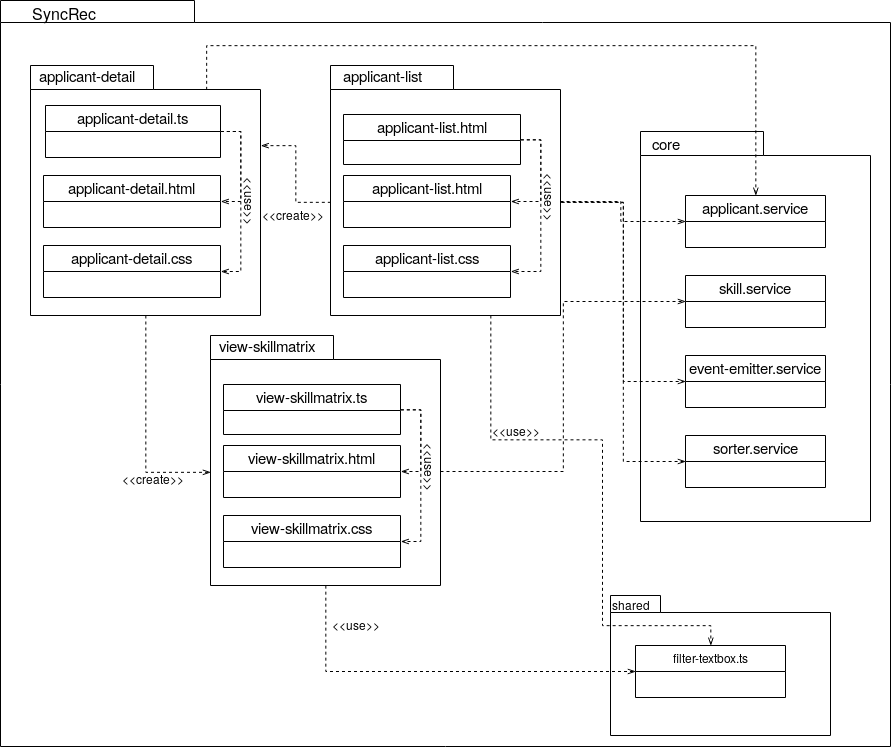
\includegraphics[width=1\columnwidth]{immagini/usecase/UML1} 
	\caption{Struttura dei component sviluppati per l'applicativo SyncRec}
	\label{figura:UML1}
\end{figure}


Come già accennato in precedenza, \hyperref[angular]{Angular} suggerisce di applicare una forte struttura modulare alle proprie \textit{web-application}, tale approccio è stato nella gran parte perseguito, con alcune eccezioni per determinati elementi condivisi fra più \textit{component}; un'applicazione di tale struttura, inoltre, permette lo sviluppo delle proprie componenti senza dover necessariamente conoscere l'intera architettura nel dettaglio.

La figura \ref{figura:UML1} illustra la struttura dei component sviluppati per l'applicativo SyncRec, a scopo di sintesi sono state omesse alcune parti proprie del \textit{framework} di riferimento (come i moduli e gli \textit{asset}) o sviluppate da altri studenti nel corso del progetto.\\
I moduli \textit{applicant-list}, \textit{applicant-detail} e \textit{viewskillmatrix} rappresentano i componenti grafici dell'applicazione, il modulo \textit{shared} rappresenta l'insieme di \textit{component} condivisi nel \textit{namespace} globale e il modulo \textit{core} contiene i \textit{service}; quest'ultimi hanno il duplice scopo di recuperare i dati dal \textit{Back-end} e di fornire alcuni metodi di utilità necessari a svolgere determinate operazioni (come l'ordinamento o l'emissione di eventi verso \textit{components} padri).\\
La figura \ref{figura:UML2} illustra come il modulo \textit{service} si occupa di dialogare con il \textit{Back-end} scritto in \hyperref[tech-spring]{Spring}.\\
In ambito di progettazione, dialogando con gli altri laureandi che hanno preso parte alla realizzazion di SyncRec, si sono definite alcune linee guida da perseguire nel corso della codifica.\\
Tali linee guida sono:
\begin{itemize}
	\item Utilizzare il più possibile le direttive \hyperref[angular]{Angular} (come \gls{ng-Model}) all'interno del \textit{HTML} dei \textit{component}.
	\item Definire per ciascun \textit{component} il relativo modulo di referimento, tale prassi è fortemente consigliata dalla documentazione di \hyperref[angular]{Angular}.
	\item Per quanto riguarda il \textit{CSS}, favorire l'utilizzo della versione 3.0 piuttosto che della libreria esterna \textit{bootstrap}.
\end{itemize}

\begin{figure}[!h] 
	\centering 
	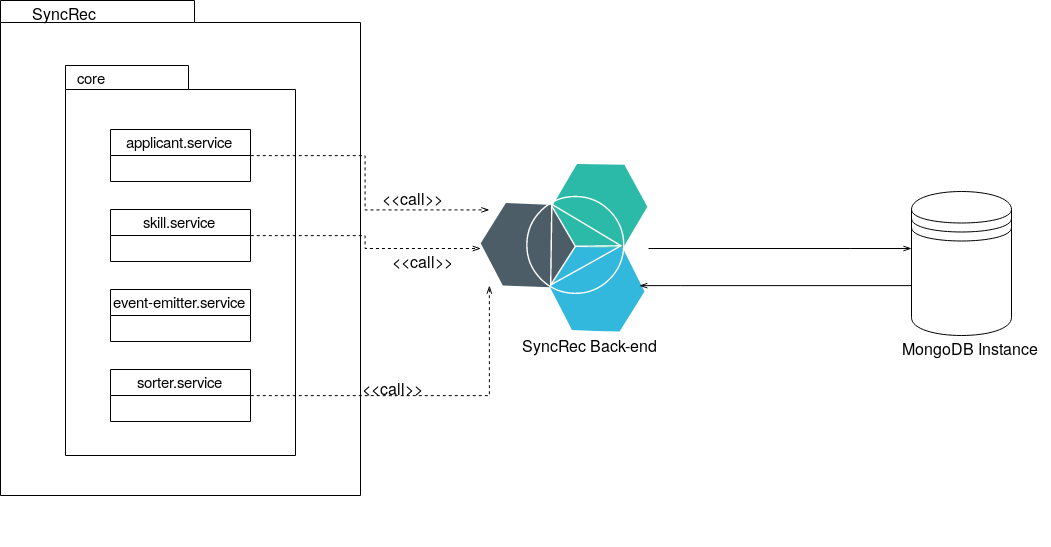
\includegraphics[width=1\columnwidth]{immagini/usecase/UML2} 
	\caption{Integrazione tra Front-end e Back-end}
	\label{figura:UML2}
\end{figure}

\subsection{Homepage}
La homepage dell'applicativo (v. figura \ref{figura:homepage}) si presenta come un semplice \textit{menù} con 3 voci.
\begin{itemize}
	\item \textbf{Aggiungi persone} reindirizza verso il \textit{component} adibito all'aggiunta degli \textit{applicant};
	\item \textbf{Visualizza persone} reindirizza verso il \textit{component} adibito alla visualizzazione della lista degli \textit{applicant}, sviluppato dal laureando nel corso del progetto di stage;
	\item \textbf{Ricerca Persone} reindirizza verso il component adibito alla ricerca delle persone;
\end{itemize}
In aggiunta, è possibile effettuare il \textit{logout} con un pulsante posto in alto, vicino al logo.
\vspace{0.5em}
\begin{figure}[!h] 
	\centering 
	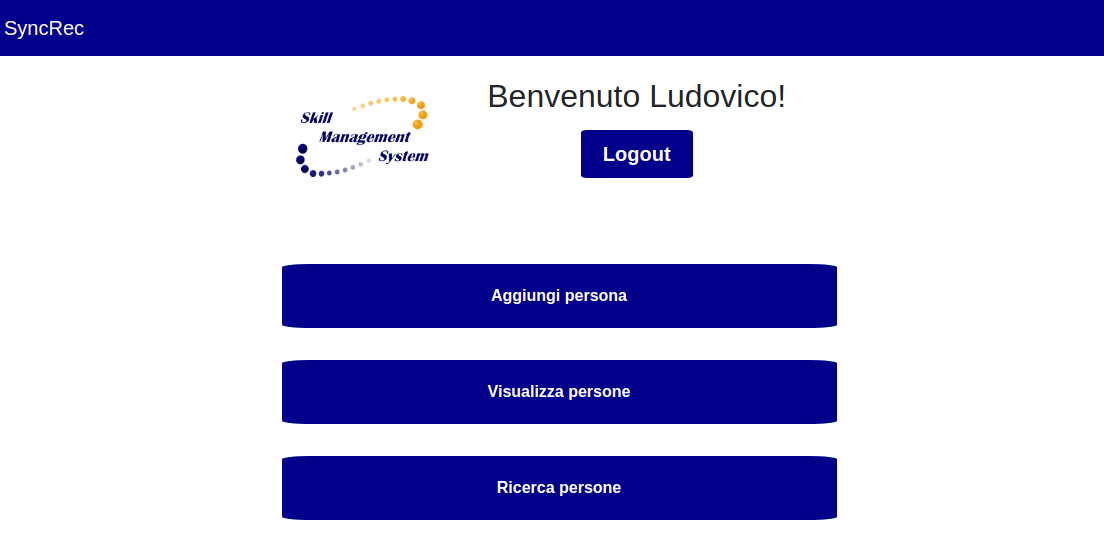
\includegraphics[width=1\columnwidth]{immagini/svil/homepage} 
	\caption{Schermata della homepage}
	\label{figura:homepage}
\end{figure}

\subsection{Maschera della visualizzazione degli\applicant} \label{section: applicant-list}
La fugura \ref{figura:lista}, mostra il \textit{component} sviluppato per la visualizzazione degli \textit{applicant}, per ciascun \textit{applicant} viene visualizzato il Cognome, Nome e l'email, insieme a un tasto per l'eliminazione e uno per la visualizzazione del dettaglio della persona, il quale reindirizza verso la maschera descritta nella sezione \ref{m-CRUD}.\\
Per realizzare questa \textit{task}, è stato necessario reperire le informazione tramite un service definito appositamente, il quale effettua una semplice GET al relativo microservizio sviluppato nel Back-end (v. codice \ref{get-applicant}).
Successivamente, i dati vengono memorizzati in un apposito \textit{array} e visualizzati tramite una direttiva \hyperref[angular]{Angular} chiamata \textit{ng-for} (v. \textit{listing}  \ref{ng-for}).

\vspace{0.5em}
\begin{figure}[!h] 
	\centering 
	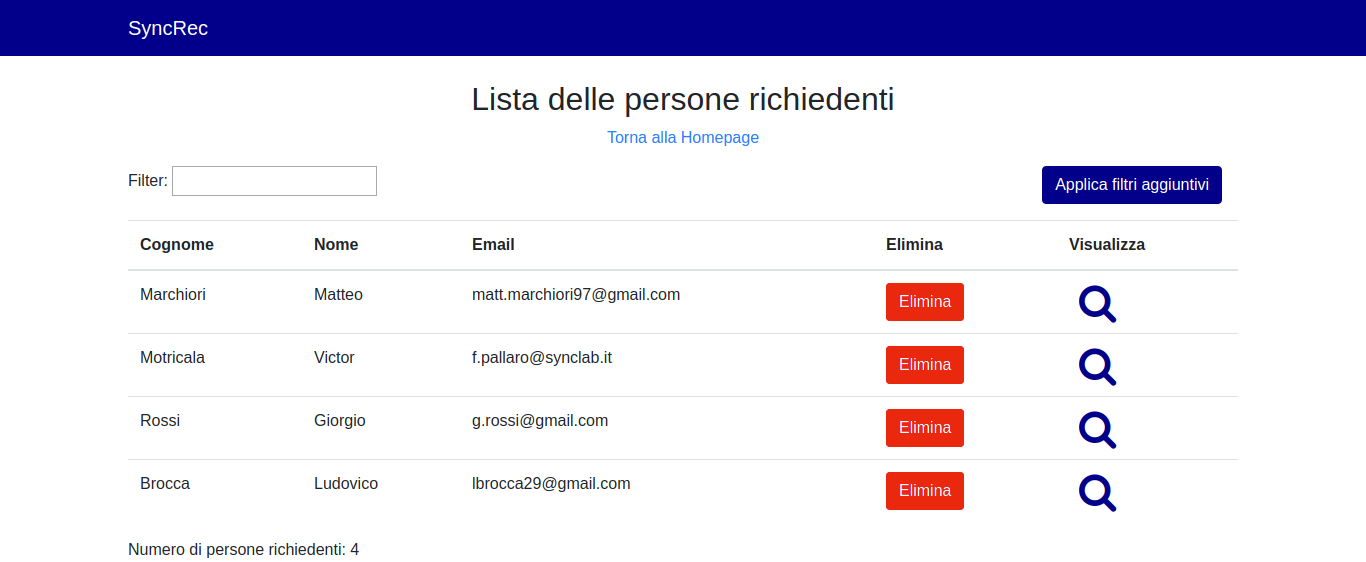
\includegraphics[width=1\columnwidth]{immagini/svil/lista} 
	\caption{Schermata della visualizzazione lista degli applicant}
	\label{figura:lista}
\end{figure}

\begin{lstlisting}[label=get-applicant,caption=Funzione del service che effettua la chiamata GET]
getAllApplicants(): Observable<Applicant[]> {
	return this.http.get<Applicant[]>(this.baseUrl).pipe(
		catchError(this.handleError)
	);
}
\end{lstlisting} 

\begin{lstlisting}[label=ng-for,caption=Visualizzazione degli applicant nel codice HTML]
<tr class="hover-tr" *ngFor="let appl of filteredApplicants;" >
	<td>
		{{ appl.surname }}
	</td>
	<td>
		{{ appl.name }}
	</td>
	<td>
		{{ appl.email }}
	</td>
	<td>
	<button class="btn" id="btn-delete-applicant-list"
		(click)="deleteApplicant(appl.id)">Elimina</button>
	</td>
	<td>
	<span class="immagineEsterna" (click)="routerRedirect(appl.id)"><i class="fa fa-search fa-2x"></i></span>
	</td>
</tr>
\end{lstlisting} 

Il pulsante posto in alto a destra visualizza il component adibito all'applicazione di filtri aggiuntivi sul totale degli applicant, come si può vedere in figura \ref{figura:filtri}.\\
Posti sopra la tabella, inoltre, è possibile visualizzare un campo di testo, che permette di filtrare i risultati secondo il nome, cognome o email. Tale filtro dinamico è stato ottenuto tramite l'azione congiunta di un service (v \textit{listing}. \ref{event-e}) e di un \textit{component} costituito da un singolo campo di testo; il \textit{component} padre in questo modo può applicare il filtro sugli applicant ogni qualvolta il contenuto del campo di testo viene cambiato (v \textit{listing} \ref{filter}), in modo simile a quanto accade con l'\gls{Observer Pattern}.

\begin{lstlisting} [label=event-e, caption= Event-Emitter service]
export class EventEmitterService {

	invokeFirstComponentFunction = new EventEmitter();
	// variabile per la sottoscrizione di un component per la // reazione  ad eventi lanciati
	subsVar: Subscription;

	constructor() { }

	onComponentAction() {
		this.invokeFirstComponentFunction.emit();
	}
}
\end{lstlisting}

\begin{lstlisting} [label=filter, caption= Funzione che filtra i dati degli applicant]
filter(data: string) {
	if (data) {
		this.filteredApplicants = this._applicants.filter((applicant: Applicant) => {
			return applicant.name.toLowerCase().indexOf(data.toLowerCase()) > -1 ||
			applicant.surname.toLowerCase().indexOf(data.toLowerCase()) > -1 ||
			applicant.email.toLowerCase().indexOf(data.toLowerCase()) > -1;
		});
		} else {
		this.filteredApplicants = this._applicants;
	}
}

\end{lstlisting}

La visualizzazione del \textit{component} relativo all'aggiunta di filtri aggiuntivi viene gestita tramite una semplice direttiva \hyperref[angular]{Angular} chiamata \textit{Ng-if}, la quale si lega a una variabile booleana e determina la visualizzazione o meno del \textit{component} a seconda del valore assegnato. La selezione dei valori, invece, viene gestita tramite i \textit{form} \hyperref[angular]{Angular}, i quali legano i valori contenuti nei vari \textit{widget} a delle strutture che gestiscono autonomamente valori di default, validazione, \textit{submit} dei risultati e quant'altro, rendendo la struttura molto solida, sicura e poco soggetta a errori.
Nel \textit{listing} \ref{form} è possibile vedere l'inizializzazione del \textit{FormBuilder}, la sopracitata struttura in grado di gestire i dati di un \textit{form}, notare che viene inserito un pattern per la validazione ove necessario.
\newpage
\begin{lstlisting}[label= form, caption= Inizializzazione di un FormBuilder]


this.filterGroup = this.formBuilder.group({
	sesso: [''],
	name: ['',  Validators.pattern('^[a-zA-Z]*$')],
	surname: ['',  Validators.pattern('^[a-zA-Z]*$')],
	qualification: [''],
	seniority: [''],
	ambito: [''],
	geodisp: this.formBuilder.array([]),
	skill: [''],
	skillLevel: [''],
	scartato: [false],
});

\end{lstlisting}

\vspace{0.5em}
\begin{figure}[!h] 
	\centering 
	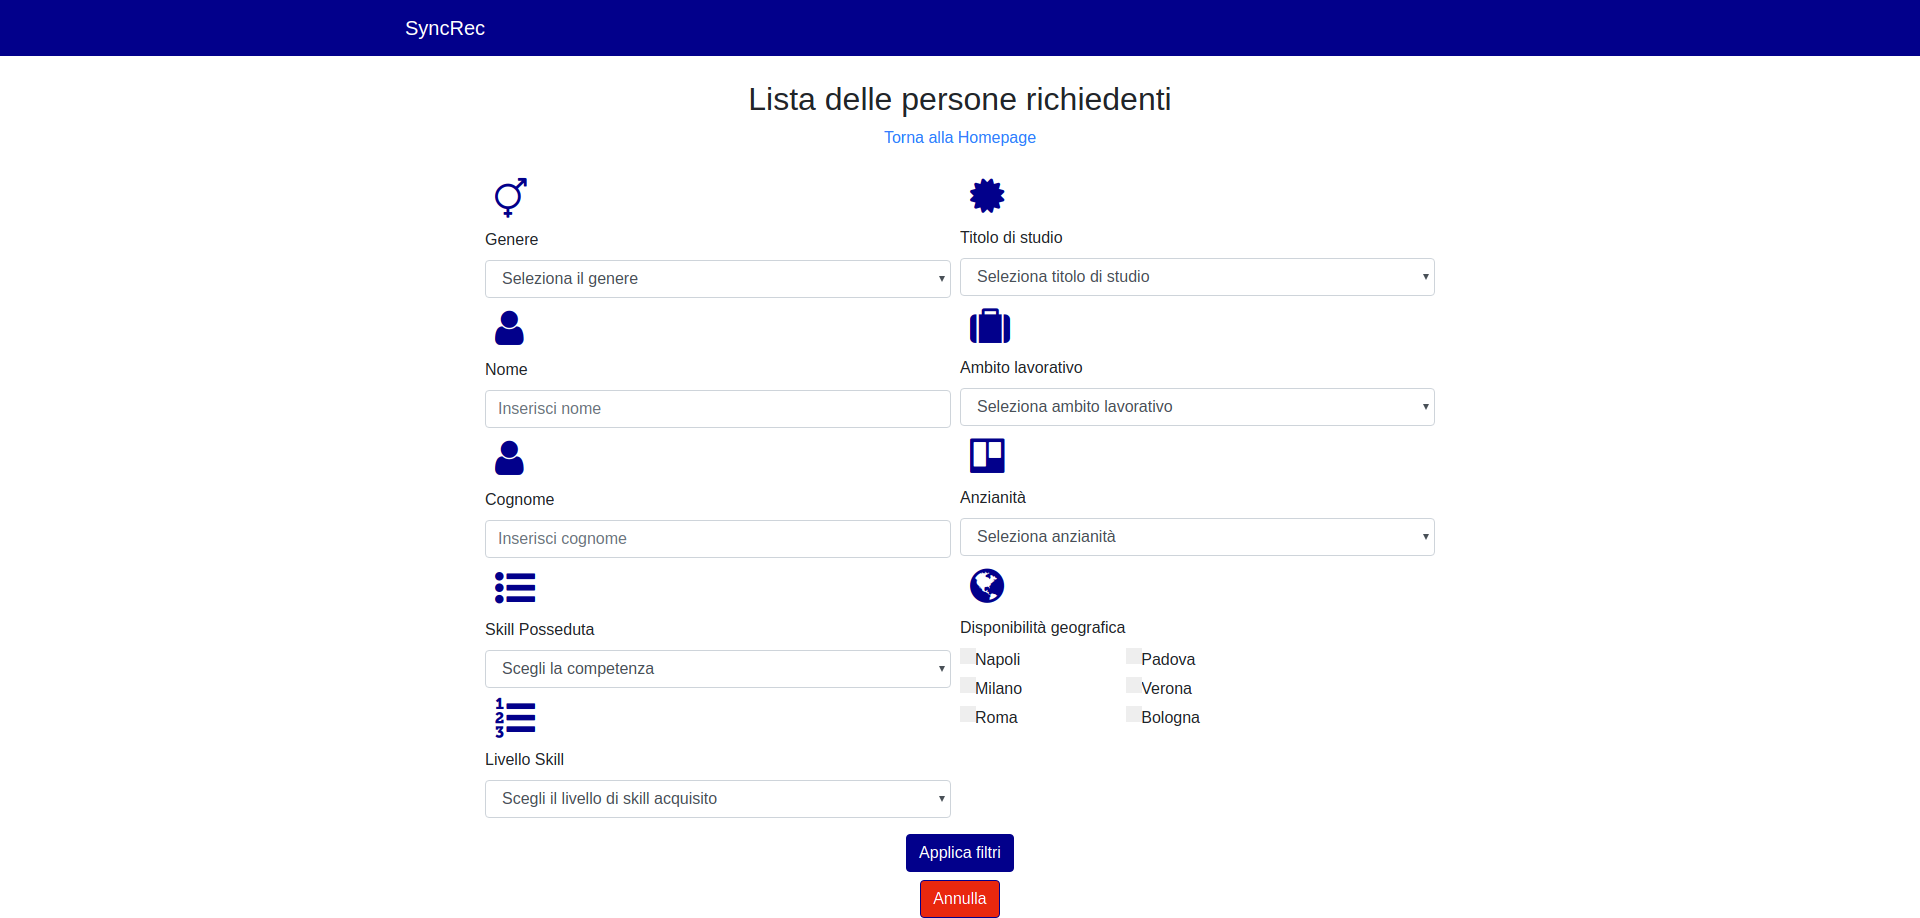
\includegraphics[width=1\columnwidth]{immagini/svil/filtri} 
	\caption{Schermata della selezione dei filtri da applicare alla lista degli applicant}
	\label{figura:filtri}
\end{figure}

\subsection{Maschera delle operazioni CRUD su un\applicant}\label{m-CRUD}
\vspace{0.5em}
\begin{figure}[!h] 
	\centering 
	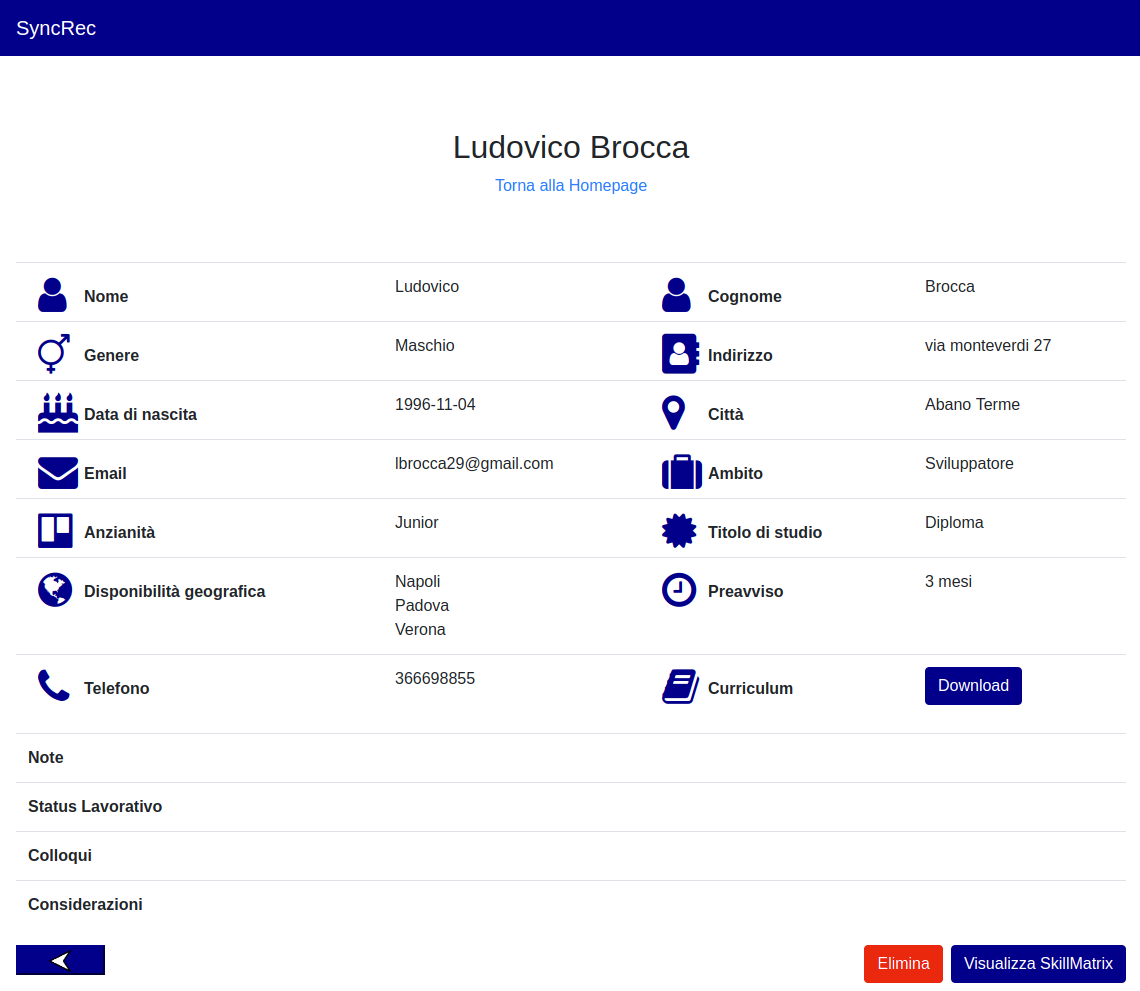
\includegraphics[width=1\columnwidth]{immagini/svil/applicant}
	\caption{Maschera CRUD del singolo applicant}
	\label{figura:applicant}
\end{figure}
La gestione delle operazioni \gls{CRUD} di un \textit{applicant} avviene tramite la maschera visible nella figura \ref{figura:applicant}; l'approccio adottato è molto simile a quanto avviene con la gestione della maschera per la selezione dei filtri aggiuntivi descritta nella sezione \ref{section: applicant-list}: viene utilizzato un \textit{FormBuilder} per la gestione dei singoli valori di un \textit{applicant}, una volta modificati, un controllo su un parametro dei \textit{FormControl}, chiamato \texttt{touched}, permette la visualizzazione dei tasti di conferma o annullamento delle modifiche, in caso di conferma viene effettuata una chiamata \textit{PUT} tramite l'apposito servizio (descritta nel \textit{listing} \ref{PUT-call}), in caso contrario vengono ripristinati i valori antecedenti alle modifiche apportate dall'utente.\\
\newpage
\begin{lstlisting}[label=PUT-call, caption=chiamata PUT al microservizio del Back-end di SyncRec]
putApplicant(applicant: Applicant): Observable<any> {
	return this.http.patch(this.baseUrl + '/' + applicant.id, applicant).pipe(
		catchError((err: HttpErrorResponse) => {
			if (err.error instanceof Error) {
				// A client-side or network error occurred.
				const details = {detail: err.error, status: err.status};
				return throwError(details);
			} else {
				// The backend returned an unsuccessful response code.
				const details = {detail: err.error, status: err.status};
				return throwError(details);
			}
		})
	);
	
}
\end{lstlisting}
Con i pulsanti posti in basso è possibile tornare indietro, eliminare un \textit{applicant} (tramite una chiamata DELETE al microservizio di Back-end), o visualizzare l'insieme di competenze possedute tramite l'apposita maschera descritta nella sezione \ref{section:skillmatrix}
\vspace{0.5em}.

\subsection{Maschera di visualizzazione di uno skillmatrix}\label{section:skillmatrix}
\begin{figure}[!h] 
	\centering 
	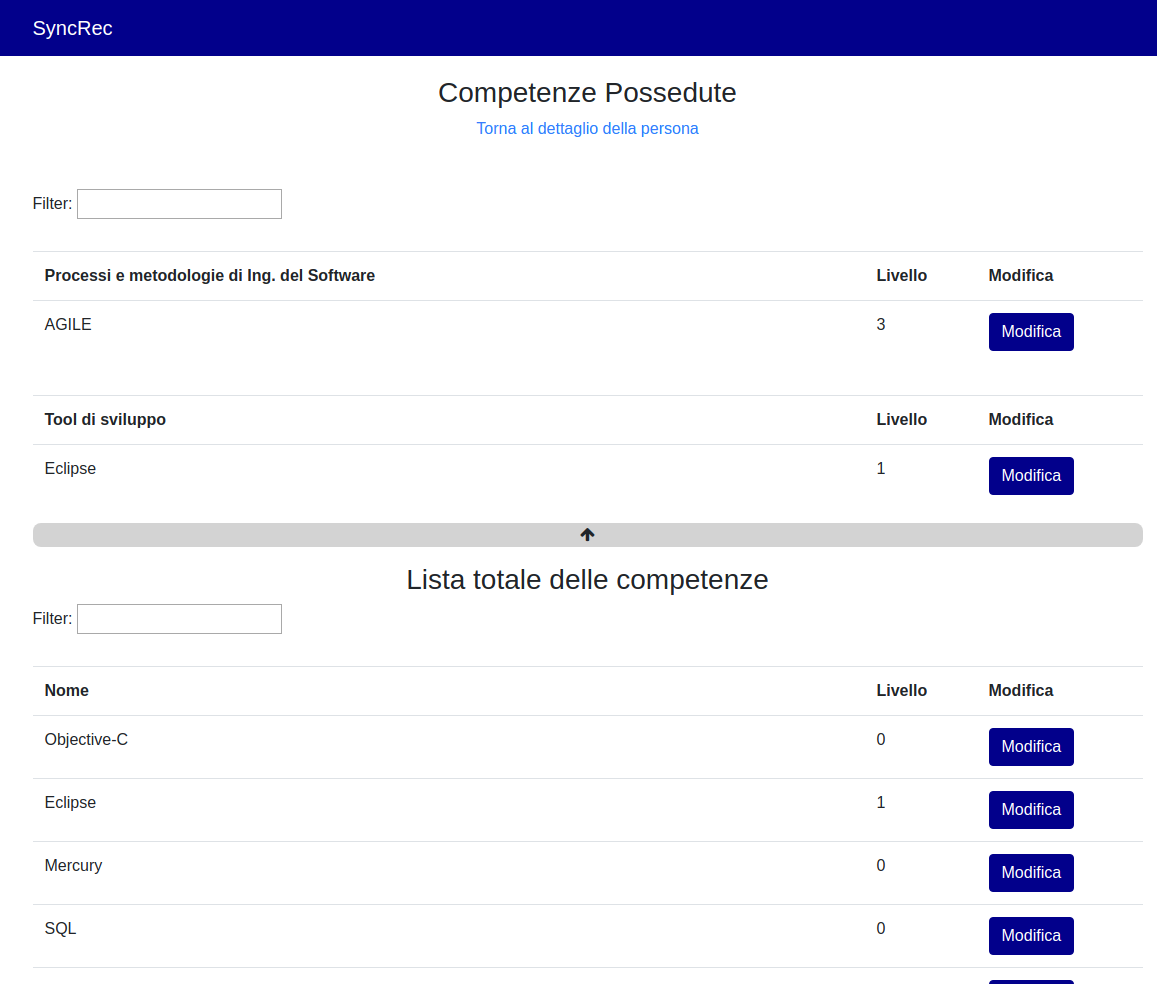
\includegraphics[width=1\columnwidth]{immagini/svil/skillmatrix} 
	\caption{Maschera CRUD dello skillmatrix}
	\label{figura:skillmatrix}
\end{figure}
Uno \textit{skillmatrix} rappresenta l'insieme delle competenze possedute da un \textit{applicant} insieme al relativo livello, che può variare da 0 a 5; una competenza per essere considerata posseduta deve avere un livello $\geq  5$.\\
\'E importante evidenziare come all'interno di SyncLab le competenze prese in considerazione siano molto numerose e tra le più disparate: nel contesto del progetto esse sono suddivise in categorie e il loro numero complessivo supera 130; ciò ha richiesto la formulazione di una soluzione che rendesse immediatamente visibile il distacco fra \textit{skill} possedute o meno e che al contempo  permettesse di modificare i valori in modo rapido.\\
Come si può vedere nella figura \ref{figura:skillmatrix}, l'approccio adottato prevede la predisposizione di 2 tabelle, una immediatamente visibile contenente l'insieme di \textit{skill} possedute per ciascuna categoria e una visibile tramite la pressione di un tasto, contenente il totale delle \textit{skill} considerate. La visualizzazione delle skill è legata alla funzione \ref{categ}, che restiuisce un booleano a una direttiva \textit{Ng-If} all'interno del codice \textit{HTML}; la quale determina la visualizzazione o meno del codice afferente al \textit{tag} legato alla direttiva, come si può vedere nel \textit{listing} \ref{skVis}.\\
\newpage
\begin{lstlisting}[label=categ, caption=Funzione che determina la visualizzazione di una categoria avente \textit{skills} possedute ]

hasThisCategorySkills(cat: string): boolean {
	let result = false;
	const category: Category = this.catalog.filter ((c: Category) => c.name === cat)[0];
	category.skills.forEach((categoryskill) => {
		this.skills.filter((sk: Skill) => {
			if (categoryskill.name === sk.name && sk.level > 0) {
				result = true;
			}
		});
	});
	return result;
}

\end{lstlisting}

Per facilitare la navigazione fra le due tabelle, viene aggiunto il \textit{component} per il filtraggio dei dati, adottando lo stesso approccio della maschera di visualizzazione lista degli \textit{applicant} (v. sez. \ref{section: applicant-list}).\\
La modifica avviene tramite un menù a tendina visibile tramite la pressione di un tasto "Modfica", la tabella di \textit{skill} possedute si aggiorna in conseguenza alla conferma del nuovo dato selezionato (aggiungendo o togliendo righe a seconda del livello della \textit{skill}).\\
Allo scopo di rendere i dati consistenti fra le due tabelle (in modo da evitare che i livelli risultino discordanti),viene utilizzato un singolo \textit{FormBuilder} e una singola struttura dati che tenga traccia dei valori per il \textit{submit} delle modifiche.\\
 
 
 \begin{lstlisting} [label=skVis, caption= HTML e direttiva Ng-If]
 <ng-container *ngIf="hasThisCategorySkills(catalog[0].name)">
 <!-- direttiva che lega al FormBuilder del component -->
 <form [formGroup]="skillGroup">
 <!-- visualizzazione HTML di una tabella -->
 </form>
 </ng-container>
 \end{lstlisting}
                % 
%% !TEX encoding = UTF-8
% !TEX TS-program = pdflatex
% !TEX root = ../tesi.tex

%**************************************************************
\chapter{Conclusioni}
\label{cap:conclusioni}
%**************************************************************

\section{COnsiderazioni generali}


\section{Obbiettivi raggiunti}

\section{Vantaggi riscontrati}

\section{Svantaggi riscontrati}

\section{Conoscenze acquisite}

\section{Sviluppi futuri}             %
%\appendix                               
%% !TEX encoding = UTF-8
% !TEX TS-program = pdflatex
% !TEX root = ../tesi.tex

%\epigraph{Citazione}{Autore della citazione}

%**************************************************************
\chapter{Altre tecnologie} \label{Appendice-1}
%**************************************************************

Lo scopo di questa sezione è fornire una panoramica delle tecnologie studiate durante il periodo di stage e previste nel piano di lavoro e che non hanno trovato un'applicazione concreta nel contesto del progetto SyncRec.\\
Tali tecnologie sono state incluse con il duplice scopo di ampliare il bagaglio di conoscenze del laureando e comprendere meglio l'architettura del progetto sul quale andavano fatti gli interventi concordati.

\section{Oracle PL/SQL} \label{plsql}
\textit{Oracle PL/SQL} è un linguaggio sviluppato da Oracle negli anni '80, si tratta di un linguaggio procedurale in grado di eseguire \textit{query SQL} insieme ad alcune strutture molto simili a quanto si può trovare in altri linguaggi procedurali (come \gls{Python} o \gls{ADA}).
PL/SQL fornisce le seguenti strutture:
\begin{itemize}
	\item Gestione degli errori;
	\item Tipizzazione dei dati;
	\item Le classiche strutture della programmazione (cicli, blocchi condizionali, funzioni etc.);
	\item Procedure;
	\item PSP (PL/SQL Server Pages);
	\item Piena integrazione con SQL(direttive DDL e DML sono disponibili in modo statico e dinamico)
\end{itemize}

\subsection{Struttura di uno script Oracle PL/SQL}
Uno \textit{script Oracle PL/SQL} è sempre suddiviso in al più tre parti:
\begin{itemize}
	\item \textbf{DECLARE:} si tratta di una sezione opzionale che contiene la dichiarazione di variabili, cursori e quant'altro;
	\item \textbf{BEGIN/END:} sezione obbligatoria che esegue le operazioni PL/SQL richieste;
	\item \textbf{EXCEPTION:} sezione facoltativa che si occupa della gestione degli errori all'interno dello \textit{script}.
\end{itemize}

All'interno del blocco \textit{DECLARE} è possibile definire inoltre due tipi di strutture: \textit{procedure} e \textit{funzioni}, dove l'unica differenza è che le seconde possono fornire valori in output tramite la keyword \textit{RETURN}.

Ogni script viene poi eseguito tramite la keyword \textit{Execute}.

\subsubsection{Cursori}
Per processare dichiarazioni SQL Oracle fornisce un area di memoria conosciuta come \textit{context area}, i \textit{cursori} costituiscono dei puntatori a tale area di memoria.\\
Il set di tuple risultanti da un'operazione SQL e puntato da un cursore è definito come l' \textit{Active Set}.\\
Per ogni operazione eseguita, Oracle instanzia un un cursore implicito, ed è inoltre possibile definire dei cursori \textit{custom} che processano le tuple una alla volta, applicando determinate trasformazioni definite dal programmatore.
I cursori vengono definiti nei blocchi PL/SQL e restringono la \textit{context area} tramite delle classiche \textit{SELECT} in SQL.\\
I cursori, in ultima analisi, sono uno strumento molto potente per manipolare i risultati delle operazioni SQL, tuttavia oggi risultano piuttosto datati se si considerano le potenzialità dei moderni \gls{framework} e la loro capacità di processare i dati contenuti nei database.

\section{Archittetture a microservizi}\label{micro}
Un’architettura basata su microservizi viene aplicata nella realizzazione di un’applicazione, essa è costituita da componenti indipendenti che eseguono ciascun processo applicativo come un \textbf{servizio}.\\
Tali servizi comunicano attraverso un’interfaccia ben definita che utilizza API leggere. Ciò risulta vantaggioso poiché ciascun componente viene eseguito in modo indipendente, e ciascun servizio può essere aggiornato, distribuito e ridimensionato per rispondere alla richiesta di funzioni specifiche di un’applicazione.\\
Ciascun servizio è progettato per una serie di capacità e si concentra sulla risoluzione di un problema specifico. Se, nel tempo, gli sviluppatori aggiungono del codice aggiuntivo a un servizio rendendolo più complesso, il servizio può essere scomposto in servizi più piccoli.

Tra le principali qualità di un'architettura a microservizi troviamo:

\begin{itemize}
	\item \textbf{Agilità:}I microservizi promuovono le organizzazioni di team indipendenti di dimensioni ridotte che diventano proprietari del servizio che gestiscono. Ciò comporta tempi di sviluppo minori in contesti ridotti e ben delineati.
	\item \textbf{Scalabilità e flessibilità}I microservizi consentono di scalare ciascun servizio in modo indipendente per rispondere alla richiesta delle funzionalità che l'applicazione supporta. Ciò permette ai team di adattare in modo corretto l’infrastruttura rispetto alle necessità, con la possibilità di monitorare accuratamente i servizi nel caso in cui essi rilevino un aumento del flusso di transazioni.
	\item \textbf{Semplicità di distribuzione}I microservizi supportano l’integrazione continua e la distribuzione continua; l'apporto di modifiche errate non inficia sul corretto funzionamento generale dell'applicazione e gli errori influiscono di meno sul costo delle operazioni. 
	\item \textbf{Libertà tecnologica} L'utilizzo di un'architettura a microservizi non è legata a un particolare \textit{stack} tecnologico: i team di sviluppo hanno piena libertà nella scelta e adozione delle tecnologie da utilizzare nel corso dello sviluppo di un progetto.
	\item \textbf{Codice riutilizzabile} La suddivisione in moduli ben delineati ha il grande vantaggio di rendere il codice riutilizzabile; è possibile quindi utilizzare moduli e servizi pienamente funzionanti per lo sviluppo di componenti aggiuntivi.
	\item \textbf{Resilienza} A differenza di quanto accade in un'architettura monolitica, un errore non è in grado in alcun modo di pregiudicare il corretto funzionamento di un'applicazione; ciò è dovuto alla natura indipendente dei servizi per come sono concepitis.
	
\end{itemize}             % Appendice A

%**************************************************************
% Materiale finale
%**************************************************************
\backmatter
\printglossaries
%% !TEX encoding = UTF-8
% !TEX TS-program = pdflatex
% !TEX root = ../tesi.tex

%**************************************************************
% Bibliografia
%**************************************************************
\cleardoublepage
\begin{thebibliography}{99}
	\bibitem{site:sqlserverpricing}
	\textit{Prezzi di SQL Server - consultato 13/09/2018}\\
	\url{https://bit.ly/2rECrAS}
	
	\bibitem{site:sqlcomparison}
	\textit{Studio comparativo sulle performance di SQL Server PostgreSQL Oracle XE e MySQL - consultato 13/09/2018}\\
	\url{https://bit.ly/2MtTE8e}
		
	\bibitem{site:svnvsgit}
	\textit{Differences Between Git and SVN  - consultato 13/09/2018}\\
	\url{https://bit.ly/2p4NzWI}

	\bibitem{site:crociereregalo}
	\textit{URL del sito CrociereRegalo (parte OTA)}\\
	\url{https://www.crociereregalo.it}
		
	\bibitem{site:dataexchange}
	\textit{URL del sito CrociereRegalo (parte DataExchange)}\\
	\url{https://data.crociereregalo.it}
	
	\bibitem{site:sviluppo-crociereregalo}
	\textit{URL del sito di sviluppo CrociereRegalo (parte OTA)}\\
	\url{http://primaretetest.webpd.it/crociereregalo}
	
	\bibitem{site:sviluppo-dataexchange}
	\textit{URL del sito di sviluppo CrociereRegalo (parte DataExchange)}\\
	\url{http://primaretetest.webpd.it/dataExchange}
	
	% Citazioni da glossario
	\bibitem{site:wikipediaIDE}
	\textit{Integrated development environment - consultato 18/09/2018}\\
	\url{https://bit.ly/2p4NzWI}

	\bibitem{site:api}
	\textit{Cosa sono le API e a cosa servono - consultato 18/09/2018}\\
	\url{https://bit.ly/2xm5qgq}

	\bibitem{site:webservice}
	\textit{Web Services Architecture - consultato 18/09/2018}\\
	\url{https://www.w3.org/TR/ws-arch/\#introduction}

	\bibitem{site:seo}
	\textit{Guida SEO all’Ottimizzazione per Motori di Ricerca - consultato 18/09/2018}\\
	\url{https://bit.ly/2QGWt9x}
	
	% Citazioni da glossario
	\bibitem{book:mvc}
	\textit{Advanced ActionScript 3 with Design Patterns}\\
	Joe Lott, Danny Patterson\\
	\textit{Pagina 46}

	\bibitem{site:rpc}
	\textit{Remote Procedure Call - consultato 18/09/2018}\\
	\url{https://bit.ly/2rjaUVo}

	\bibitem{site:soap}
	\textit{Remote Procedure Call - consultato 18/09/2018}\\
	\url{https://www.w3schools.com/xml/xml_soap.asp}	

	\bibitem{site:dbms}
	\textit{Data Base Management System - consultato 18/09/2018}\\
	\url{https://bit.ly/2HECZMV}

	\bibitem{site:rdbms}
	\textit{RDBMS - consultato 18/09/2018}\\
	\url{https://bit.ly/1MLo1Q4}
	
	\bibitem{site:framework}
	\textit{Framework - consultato 18/09/2018}\\
	\url{https://bit.ly/2QGe2Gr}
	

	\bibitem{site:dom}
	\textit{JavaScript HTML DOM - consultato 18/09/2018}\\
	\url{https://www.w3schools.com/js/js_htmldom.asp}	
	

	\bibitem{site:json}
	\textit{Introducing JSON - consultato 18/09/2018}\\
	\url{https://www.json.org/}


	\bibitem{site:ajax}
	\textit{AJAX Introduction - consultato 18/09/2018}\\
	\url{https://www.w3schools.com/xml/ajax_intro.asp}
	
	% Fine citazioni da glossario
\end{thebibliography}




\end{document}
